%; whizzy chapter
% -initex iniptex -latex platex -format platex -bibtex jbibtex -fmt fmt
% 以上 whizzytex を使用する場合の設定。

%     Tokyo Debian Meeting resources
%     Copyright (C) 2010 Junichi Uekawa

%     This program is free software; you can redistribute it and/or modify
%     it under the terms of the GNU General Public License as published by
%     the Free Software Foundation; either version 2 of the License, or
%     (at your option) any later version.

%     This program is distributed in the hope that it will be useful,
%     but WITHOUT ANY WARRANTY; without even the implied warranty of
%     MERCHANTABILITY or FITNESS FOR A PARTICULAR PURPOSE.  See the
%     GNU General Public License for more details.

%     You should have received a copy of the GNU General Public License
%     along with this program; if not, write to the Free Software
%     Foundation, Inc., 51 Franklin St, Fifth Floor, Boston, MA  02110-1301 USA

%  preview (shell-command (concat "evince " (replace-regexp-in-string "tex$" "pdf"(buffer-file-name)) "&"))
% 画像ファイルを処理するためにはebbを利用してboundingboxを作成。
%(shell-command "cd image201011; ebb *.jpg")

%%ここからヘッダ開始。

\documentclass[mingoth,a4paper]{jsarticle}
\usepackage{monthlyreport}
\usepackage{supertabular}

% 日付を定義する、毎月変わります。
\newcommand{\debmtgyear}{2010}
\newcommand{\debmtgmonth}{11}
\newcommand{\debmtgdate}{20}
% (+ (* (- 2010 2005) 12) 10) started from zero
\newcommand{\debmtgnumber}{70}

\begin{document}

\begin{titlepage}
\thispagestyle{empty}
% タイトルページ:編集必要な部分は最初のマクロに飛ばすこと

\vspace*{-2cm}
第\debmtgnumber{}回 東京エリア Debian 勉強会資料\\
\hspace*{-2cm}

\includegraphics[width=210mm]{image201003/debsen.eps}\\
\hfill{}\debmtgyear{}年\debmtgmonth{}月\debmtgdate{}日

% ここはアップデートすること
\rotatebox{10}{\fontsize{32}{32} {\gt 特集: 俺のファイルシステムは熱いぜ!}}

\vspace*{-2cm}
\hfill{}
\includegraphics[height=6cm]{image200502/openlogo-nd.eps}
\end{titlepage}

\dancersection{Introduction}{上川 純一}

\begin{multicols}{2}
 

 今月のDebian勉強会へようこそ。これからDebianの世界にあしを踏み入れると
 いう方も、すでにどっぷりとつかっているという方も、月に一回Debianについ
 て語りませんか?

 Debian勉強会の目的は下記です。

 \begin{itemize}
 \item \underline{Debian Developer} (開発者)の育成。
 \item 日本語での「\underline{開発に関する情報}」を整理してまとめ、アップデートする。
 \item \underline{場}の提供。
 \begin{itemize}
  \item 普段ばらばらな場所にいる人々が face-to-face で出会える場を提供
	する。
  \item Debian のためになることを語る場を提供する。
  \item Debianについて語る場を提供する。
 \end{itemize}
 \end{itemize}		

 Debianの勉強会ということで究極的には参加者全員がDebian Packageをがりがり
 と作るスーパーハッカーになった姿を妄想しています。情報の共有・活用を通し
 て Debianの今後の能動的な展開への土台として、「場」としての空間を提供す
 るのが目的です。

\end{multicols}

\newpage

\begin{minipage}[b]{0.2\hsize}
 \definecolor{titleback}{gray}{0.9}
 \colorbox{titleback}{\rotatebox{90}{\fontsize{80}{80} {\gt デビアン勉強会} }}
\end{minipage}
\begin{minipage}[b]{0.8\hsize}
\hrule
\vspace{2mm}
\hrule
\begin{multicols}{2}
\tableofcontents
\end{multicols}
\vspace{2mm}
\hrule
\end{minipage}

\dancersection{事前課題}{上川 純一}

今回の事前課題は以下です:
\begin{itemize}
 \item 日常的に活用しているファイルシステム設定について紹介する。(例、LVM, ext3, jffs, ...)
\end{itemize}
この課題に対して提出いただいた内容は以下です。
\begin{multicols}{2}
{\small
 \begin{prework}{ ����(yy\_y\_ja\_jp) }
���ޤ���������ǤϤʤ��Ǥ���... �긵�Υ�åץȥåפǤ� /boot �ˤ� ext2
 ����¾�ˤ� ext3���Ƕ�ȤäƤ���ǥ����ȥåפǤ� /boot �ˤ� ext3 ����¾
 �ˤ� LVM ��� ext4 ��ȤäƤ��ޤ���
\end{prework}

\begin{prework}{ �����ϥ� }
�ǥե���Ȥ�ext3����
�����ǥե���ȤΤޤޡ�
(NTFS���VM���᡼�����ext3�⤢�뤱��)
\end{prework}

\begin{prework}{ yos.takahashi }
ext3/4���˻ȤäƤޤ���ext3�Υǡ�������١����ˤĤ�������Linux2011ǯ1���˼�ɮ���ޤ�����
\end{prework}

\begin{prework}{ MATOHARA }
����inode �ϳ���������Ƥ���inode ��ưŪ�˳�����Ƥ���XFS �����򤹤뤳
 �Ȥ�¿���Ǥ���NILFS �Ͼ�����Ƥߤ��ΤǤ�����mount ���˰ʲ��Τ褦�ʥ��
 ���������ФƤޤ��ݤ��ʤȻפ��ޤ�����
\begin{commandline}
$ sudo mount /dev/sdb1 /mnt
mount.nilfs2: WARNING! - The NILFS on-disk format may change at any time.
mount.nilfs2: WARNING! - Do not place critical data on a NILFS filesystem. 
\end{commandline}
����¾NotePC �Ǥ�dm-crypt �ξ�˥ե����륷���ƥ���֤��ưŹ沽�����ꡢ
 eCryptfs �ǰŹ沽�����ꤷ�Ƥ��ޤ����񤭹��߻���CPU �򤫤ʤ���񤷤ޤ��ġ�
\end{prework}

\begin{prework}{ ��ޤ� }
��ext2-$>$reiserfs-$>$jfs-$>$xfs-$>$reiserfs-$>$ext3�ȻȤäƤ��ޤ�����

����:
\begin{itemize}
 \item reiserfs: ���ե������¿���ե�����Υ������������ӥ��Ӥ��Ƥ��ɤ���
       �����������դȤ����ⵤ�������θ�μ�žȬ�ݥ����ɤˡ�����
 \item jfs: ����v1.0��̾��ä�IBM���ꥨ�ʥ��������ˤ�xfs��ƨ��
 \item xfs: fsck==true�˴�ư����������ǯ�Ȥä���ΤΥޥ�����Ĵ����0byte
       �ե��������������Ѥ���줺ƨ����
\end{itemize}
������reiser4��Ķ���Ԥ��뤦���ˤ��줬�����ʤäơ����ext3�˸��경��htree�����ä������⤦Ŵ�Ĥʤ鲿�Ǥ⤤���Ǥ��������Ȥ����Ĥ�nilfs�ʤɤ˼��Ф��Ƥ��ޤ���ext3�������noatime���٤Ǥ����������aufs���碌�Ƽ�ʬ���Ȥ��Ȥ� *strap �Ķ��򥯥����˥󥰤��Ƥ��ޤ����¸����ƥ��Ȥ������Ǥ�����Ǥ���USB�����ư�Ǥ�ͭ�ѡ�

���LVM�ǤϤʤ�MD��Ȥäƾ�Ĺ���ܥХå����åפ򤷤Ƥ��ޤ���
 MD(sda,sdb,sdc)�ǹ��ۤ����̾��MD(����)�Dz�ư���Хå����åפλ���
 attach/detach�򤹤롣�֥��å���٥�ʤΤǥꥫ�Х��FSǤ���Ǥ��������̤�
 �������¾����ˡ���ʤ�������
\end{prework}

\begin{prework}{ henrich }
�ȤäƤ���֤�NTFS��Ĺ���󤸤�ʤ��Ǥ����͡����졣
�����Ρ����Ѥο������ǥ�������ext4�ǥե����ޥåȤ��ޤ����������㤤��Ƚ��ʤ��Ȥ����������Ƥ��ޤ���
\end{prework}

\begin{prework}{ emasaka }
�Ĥ뤷��FS��ȤäƤޤ�
\end{prework}

\begin{prework}{ �ܾ� }
ext3����Ѥ��Ƥ��ޤ����ä��Ѥ�ä����ȤϤ��Ƥ��ޤ���
FS����ʤ��Ǥ������Ƕ�Lenny��2TB��HDD��Ȥä���parted�äƤλȤ��ƶä��ޤ�����
\end{prework}

\begin{prework}{ ����@������ }
���������Ū�˳��Ѥ��Ƥ���ե����륷���ƥ��ReiserFS�Ǥ���
�Ż��ǻȤäƤ�Ķ���ext3�Ǥ�����ext3���Ÿ������ǥ��㡼�ʥ뤬
����Ʋ��Ǥ������ηи��ʸŤ������ͥ�Ǥ���...�ˤ����ꡢ
���ޤ꿮�Ѥ��Ƥ��ޤ���
�����ReiserFS�Ķ��ǤϤ���ޤǤνꤤ���ʤ��Ÿ����ڤä��ꡢ
�Ƥ�HDD�����줫�����ꤷ�Ƥ��ﳲ����ä��и���̵���Τǡ�
��³Ū�˻ȤäƤ��ޤ���
��ǯ����ReiserFS�Υᥤ��ȯ��(Hans Reiser)�����ᤵ��Ƥ��ޤ������ƥʥ󥹤��ۤ��Ƥ��ޤ�����
�����������θ��ReiserFS��¾�γ�ȯ�Ԥˤ���³�����ݼ餵��Ƥ���Τǡ��¿����ޤ�����
\end{prework}

\begin{prework}{ nozzy123nozzy }
\begin{enumerate}
 \item LVM�ˤĤ��Ƥϡ�CentOS5.5��Ƴ�������Τ��Τޤޤ����Ѥ��Ƥޤ�����
       ���������ƥब��äƤ���Volume̾�ϥǥե���Ȥ�����ȡʼºݤˤ�
       kickstart�ˤơˤ��ѹ����ƻȤäƤޤ����ʾ㳲���Υ���١����˺��뤿
       ���
\item ext3�ˤĤ��Ƥϡ�debian-sid�����Τޤ޻��ꤷ�Ƥ����Τ򤽤Τޤ޻Ȥ�
      �Ƥ����ꤷ�ޤ���relatime, noatime ���餤�Ͼ����ɲä��Ƥߤ����ʡ���
      �ϻפäƤޤ���
\end{enumerate}
\end{prework}

\begin{prework}{ �ޤ��������ؤ� }
\begin{itemize}
 \item Debian�Ǥ��ä˶Ťä����Ȥ�����ext3��ȤäƤޤ������ۥޥ����qcow2
       ���᡼���ǥ��������ѻ��ʳ��ϡ�LVM�ϻȤäƤޤ���
 \item �����ǰ����ü�ʤΤϡ��������DHCP�������Ѥ�Armadillo-J�ǻȤäƤ�
       ��JFFS�Ǥ����ǥե���ȤΥե����०�����Ǥϥ�֡��Ȥ�����������
       �ƽ��������Ƥ��ޤ��Τǡ�RAM�ΰ�˽񤭤��ߡ��Ÿ��ڤäƤ�ä��ʤ�
       ���������Ǥ���Debian��udhcp�Υ������ѥå���������ӥ�ɤ��ƻȤäƤޤ���
       \footnote{\url{http://d.hatena.ne.jp/mkouhei/20080601/1212330630}}
 \item ��Debian���ߤǡ���ʬ����ǰ��֥ۥåȤʤΤ�palm webOS�Ǥ��������Ubuntu��
       �������ޥ���������Τ餷���ΤǤ�����/etc/mtab�򸫤��35�Ԥ⤢�ꡢ
       ���ʤ����֤ʹ����Ǥ��͡�
\end{itemize}
\end{prework}
}
\end{multicols}

\dancersection{最近のDebian関連のミーティング報告}{まえだこうへい}
\subsection{東京エリアDebian勉強会69回目報告}

久々の通常どおりのDebian勉強会は10/16に、場所は大森のニフティさんのセミ
ナールームをお借りして開催しました。勉強会のサイトでは第69回となっていま
すが、8月は開催していないので今回は正確には68回です*1。鯖読んでます。
が、68回は欠番としました。

\subsubsection{開催内容}
今回は最近のイベント、とくにLinuxCon Japan 2010とDebconf10の参加報告のあ
と、事前課題の「俺のDebianな一日」を参加者全員に自己紹介を兼ねて発表して
貰い、日本でのMini Debconf開催に向けてのブレストを行いました。今回初参加
のhattorinさんとtanさんが次回ネタを発表してくれることになったこと、Mini
Confに向けてのディスカッションは次回以降も続けていくことになりました。

\subsubsection{参加者}
参加者(敬称略)は、tai、日比野、あらき、hattorin、吉野、キタハラ、小室、
山本、鈴木、あけど、やまね、上川、まえだの計13人でした。

ニフティさんありがとう!
ニフティさんには会場をお借りしただけでなく、勉強会の最後に無茶ぶりしても
きちんとコメントも頂き、誠にありがとうございました。

\subsubsection{宴会}
宴会はしゃぶしゃぶ温野菜 大森店で行いました。

% (query-replace-regexp "<.*?>" "")
% (query-replace-regexp "^[	 ]\+" "")

%-------------------------------------------------------------------------------
\dancersection{ext4 ファイルシステムをDebianで活用してみる}{上川 純一}
%-------------------------------------------------------------------------------
\index{ext4}

ext4 ファイルシステムは Linux で広く使われている ext3 の後継ファイルシス
テムとして登場したファイルシステムです。特徴としては、ext3 と同じくジャー
ナリング機能をもち、データ領域をブロック単位ではなくエクステント(一連の領
域)で確保していること。32ビットから48ビットになったので、ファイルシステム
サイズがext3 の制限を越えている。atimeなどが秒より細かい時間でわかるよう
になる、などです。\cite{ext42007,ext42008}

\subsection{ext4 ファイルシステムを作ってみる}

それでは、ext4ファイルシステムを作ってみましょう。実は通常のext3ファイル
システムをそのままext4としてマウントすることもできるようです。そうすると徐々に
ファイルが書き換えるたびにextentベースになったりするようです。
ただ、ファイルシステム全体のパラメータがext4用ではないので、ファイルシス
テムをいちから作成するのがよいでしょう。

アロケータのアルゴリズムも改善されているので小さなファイルのアロケーショ
ンも改善しているようですので、既存のファイルシステムの内容をバックアップ
してリストアするのがよいのではないでしょうか。

ext4 を使うには十分新しい e2fsprogs と十分あたらしいLinux Kernel があれば
よいです。Debian 5.0 (lenny) の時点で必要なパッケージはそろっているようです。

\begin{commandline}
 $ sudo lvcreate -L 1G -n lvext4 vghoge
  Logical volume "lvext4" created
 $ sudo mount /dev/vghoge/lvext4 /mnt/
 $ mount -v 
 /dev/mapper/vghoge-lvext4 on /mnt type ext4 (rw)
 $ df -h /mnt/
 Filesystem          サイズ  使用  残り 使用% マウント位置
 /dev/mapper/vghoge-lvext4
                     1008M   34M  924M   4% /mnt
 $ df -T /mnt/ 
 Filesystem    Type   1K-ブロック    使用   使用可 使用% マウント位置
 /dev/mapper/vghoge-lvext4
              ext4     1032088     34052    945608   4% /mnt
 $ df -i /mnt/
 Filesystem            Iノード  I使用   I残り I使用% マウント位置
 /dev/mapper/vghoge-lvext4
                       65536      11   65525    1% /mnt
\end{commandline}

\begin{thebibliography}{0}
 \bibitem{ext42007} A. Mathur, M. Cao, S. Bhattacharya, A. Dilger, A. Tomas, and
 L. Vivier. "The new ext4 filesystem: current status and future plans,"
 Linux Symposium. 2007

 \bibitem{ext42008}  A. Kumar K. V., M. Cao, J. R. Santos, and A. Dilger. "Ext4 block and inode allocator improvements," Linux Symposium, Vol 1. 2008.

\end{thebibliography}

%-------------------------------------------------------------------------------
\dancersection{NILFSをDebianで活用してみる}{山田 泰資}
%-------------------------------------------------------------------------------
\index{NILFS}
\subsection{はじめに}
NILFS
\footnote{正式にはNILFS2ですが、すでにv2が登場して久しいので
本レポートではバージョン番号は略します}
はLinuxの新型ファイルシステムの1つです。
登場自体はv1が2003年と結構前なのですが、機能を増強したv2が
2007年に登場し、その後SSD上での性能が著しく優れる\cite{nilbench}
などのニュースで注目を集め、Linux 2.6.30(2009/6リリース)で
メインラインに統合されるに至りました。

ここではnilfsの特徴・使い方を紹介し、その上で他の有力(?)な
選択肢としてのLVMおよびbtrfsとの比較を行います。

\subsection{使ってみよう - nilfsの導入と特徴}
\label{sec:try-nilfs}
nilfsは通常のファイルシステムですので、とりあえず使い始めるだけなら
簡単です。デモを兼ねてまずは使い始めましょう。

\begin{commandline}
// 8GBの領域を使います
# parted -s -a none /dev/sda mklabel gpt
# parted -s -a none /dev/sda unit s mkpart primary ext2 2048 14682112

// 普通にmkfsしてmount
# mkfs.nilfs2 /dev/sda1
mkfs.nilfs2 ver 2.0
Start writing file system initial data to the device
       Blocksize:4096  Device:/dev/sda1  Device Size:7516193280
File system initialization succeeded !!
# mount /dev/sda1 /mnt/p0
mount.nilfs2: WARNING! - The NILFS on-disk format may change at any time.
mount.nilfs2: WARNING! - Do not place critical data on a NILFS filesystem.
[2845849.612706] segctord starting. Construction interval = 5 seconds, CP frequency < 30 seconds

// さあ使ってみよう
# ls /mnt/p0
# <- 空の状態
# echo hello > /mnt/p0/file
# cat /mnt/p0/file
hello
\end{commandline}

何の変哲もないファイルシステムですね。しかし面白いのはここからです。

nilfs最大の特徴は「連続スナップショット」機能です。
\begin{quote}
\Large{スナップショットは判るけど連続って?}
\end{quote}
と思われるかもしれません。答はnilfsの固有コマンドlscpを打つと判ります:

\begin{commandline}
# lscp
CNO        DATE     TIME  MODE  FLG   NBLKINC       ICNT
  1  2010-11-12 07:03:53   cp    -         11          3
  2  2010-11-12 07:05:45   cp    -         14          4
\end{commandline}

上では2行表示されていますが、これはそれぞれの瞬間におけるnilfsの状態を
保持していますよ、という意味になります。いわゆるスナップショットです。
ただし、nilfsではスナップショット(ss)とチェックポイント(cp)と概念が
2つあります。いずれもある瞬間の状態を保持するという意味の「スナップ
ショット」である点は同じですが、運用上の扱いがやや異なります。

そして、これらの過去の状態はファイルシステムとしてそれぞれ個別に
マウントすることができます。試しに、
\begin{quote}
\Large{うっかりファイルを消してしまったけど、nilfsがチェックポイントに\\
保存してくれていたのでそれをマウントすれば回復できて安心!}
\end{quote}
というデモをやってみましょう:

\begin{commandline}
# ls /mnt/p0/
4 file0  4 file1  4 file2
# date
Fri Nov 12 07:19:14 JST 2010
# rm /mnt/p0/file2                                       <- うっかり消してしまった!どうしよう!(棒
# lscp
CNO        DATE     TIME  MODE  FLG   NBLKINC       ICNT
  1  2010-11-12 07:03:53   cp    -         11          3
  2  2010-11-12 07:05:45   cp    -         14          4
  3  2010-11-12 07:12:55   cp    -         12          5
  4  2010-11-12 07:13:21   cp    -         15          6
  5  2010-11-12 07:13:32   cp    -         27          6
  6  2010-11-12 07:16:45   cp    -         10          6
  7  2010-11-12 07:16:54   cp    -         13          6
  8  2010-11-12 07:16:56   cp    -         11          6
  9  2010-11-12 07:18:33   cp    -         13          5
 10  2010-11-12 07:19:11   cp    -         14          6 <- 消す直前の段階はCNO==10
 11  2010-11-12 07:19:18   cp    -         13          5
# chcp ss 10                                             <- スナップショットに変換する
# mount -t nilfs2 -o ro,cp=10 /dev/sda1 /mnt/p0.10       <- 消す前の状態をマウント
# ls /mnt/p0.10/
4 file0  4 file1  4 file2                                <- 消す前の状態を確認
# cp /mnt/p0.10/file2 /mnt/p0/                           <- 回復!
\end{commandline}

見ての通り、無事回復できました。nilfsは書き込みをフラッシュする度に自動的に
チェックポイントを作るので、
編集$\rightarrow$保存$\rightarrow$誤削除
などのオペミスをしても、直後ならばまず確実に復活することができます。
これは通常のスナップショットやバックアップツールにない強力な特徴です。

nilfsの管理コマンドは、このスナップショット機能を中心に整備されています。
現在あるコマンドは以下の通りです\ref{nilcmd}:
\begin{table}[h]
\begin{center}
\begin{tabular}{|r|l|}
\hline
コマンド名 & 機能 \\ \hline
mkfs.nilfs2   & nilfs(v2)ファイルシステムを作成する \\ \hline
mount.nilfs2  & マウントする \\ \hline
umount.nilfs2 & アンマウントする \\ \hline
lscp & チェックポイント・スナップショットの一覧を表示する \\ \hline
mkcp & チェックポイント・スナップショットを作成する \\ \hline
chcp & チェックポイント・スナップショットを相互変換する \\ \hline
rmcp & チェックポイントを削除する \\ \hline
lssu & ディスク上のnilfs内セグメントの使用状態を表示する \\ \hline
nilfs\_cleanerd & ガーベージコレクション処理を行う(詳細後述) \\ \hline
dumpseg & デバッグ用。nilfs内セグメントの情報をダンプする \\ \hline
\end{tabular}
\caption{nilfsの管理コマンド一覧}
\label{nilcmd}
\end{center}
\end{table}

\subsection{チェックポイント(cp)とスナップショット(ss)}
さて、チェックポイントとスナップショットの違いですが、以下の通りと
なります\ref{nilcpvsss}:
\begin{table}[h]
\begin{center}
\begin{tabular}{|r|c|c|}
\hline
 & チェックポイント  & スナップショット \\ \hline
自動的に作られるか? & YES &  NO \\ \hline
手動でも作れるか?   & YES & YES \\ \hline
自動で開放されるか? & YES &  NO \\ \hline
マウントできるか?   &  NO & YES \\ \hline
\end{tabular}
\caption{チェックポイントとスナップショットの違い}
\label{nilcpvsss}
\end{center}
\end{table}

上の実行例にてchcpコマンドで変換していましたが、チェックポイントと
スナップショットはその名称が異なるだけで、内部的には同じものです。
ただ、その名称によって自動生成・自動削除の扱いが変わり、またそれに
連動してマウントの可否も異なる、という形になります。

nilfsではチェックポイントが自動的に存在する状態が基本線で、
管理者としては永続的に残したい状態をスナップショットとして作り、
必要に応じてマウントし内容を参照する、というのが通常の使い方となります。

\subsection{nilfsの構造 - ログ構造化ファイルシステム}
nilfsは種類としてはログ構造化ファイルシステム(LFS\footnote{LFSという
名前の実装もあって、ややこしい・・・(JFSも)})の実装です。
これはext3やbtrfsなどのジャーナリングファイルシステムとは異なる設計で、
以下のような違いがあります
\footnote{と言いつつ、btrfsではジャーナルもデータ領域もextents上の
同一構造で区別がなく、書き込み処理などでもLFS的な要素を取り込んで
います\cite{nilbtrfmt}}:
\begin{itembox}[l]{ジャーナリングファイルシステムの特徴}
\begin{enumerate}
\item
書き込みはジャーナルログ領域にまず記録され、追って実際のデータ領域に反映させる
\item
クラッシュ時は、ジャーナルログを走査し、未反映分をデータ領域に反映させる
\end{enumerate}
\end{itembox}

\begin{itembox}[l]{ログ構造化ファイルシステムの特徴}
\begin{enumerate}
\item 書き込みでは元データ領域は更新せず、新たに空き部分を確保して追記する
\item クラッシュ時は、追記内容を過去に遡り、正常終了していた部分まで巻き戻す
\end{enumerate}
\end{itembox}

ジャーナリングファイルシステムではジャーナルログかデータ領域の
いずれかに必ず正当なデータが存在することになり、クラッシュ耐性の
高いファイルシステムが実現されます。デメリットは、ジャーナル領域と
データ領域に二度同じ内容を書くため、そこがオーバーヘッドとなります
\footnote{このためメタデータのみジャーナリングするなどの対応を取る}。

そして、一方のログ構造化ファイルシステムでは、元データ領域か
追記されたデータ領域のいずれかに必ず正当なデータが存在することになります。
これをジャーナリングと比較すると、
\begin{enumerate}
\item 書き込みは1回するだけなので効率がよい
\item リカバリは書き込みの末尾から最後の有効な追記部分を遡って探すだけで高速
\end{enumerate}
というメリットがあります。しかし、追記のみでは削除・書換されたファイルが
開放されず容量を消費するため、これを開放するためのガーベージコレクション
処理(GC処理)をいずれ実行する必要があり、これがオーバーヘッドとなります。

さて、nilfsは昨年頃よりSSD上でのベンチマークで高スコアを出すと報告され
注目を集めましたが、これは
\begin{itemize}
\item SSDはブロック書換えのオーバーヘッドが大きく、追記処理で最高性能を出す
\item nilfsは空きがある限りシーケンシャル書き込みでの追記になる(特に、GCが走っていない場合)
\end{itemize}
という2つの要因が合わさった事によるものです。しかし、その後
\begin{itemize}
\item SSDは追記以外の書き込み処理の効率化を進めた
\item ジャーナリング系FSもデータブロックの確保・書込方法を改良して行った
\end{itemize}
という事があり、nilfsがLFSであることをもって書き込み性能が特に優れたり、
SSDでの利用に向くという訳ではなくなってきています。特に、GC中の性能や
フラッシュメモリ上での利用において注意が必要です\cite{nilperf,nilssd}
(詳細後述)。

さて、ここら少しだけnilfsの構造を見てみることにしましょう\ref{nilfmt}。
図の通りデータは前方から並び、末尾にデータを参照するメタデータブロックが
付くだけのシンプルな構造であることが判ります。

\begin{figure}
\begin{center}
\includegraphics[width=0.8\hsize]{image201011/nilfs-graphics-001.eps}
\caption{nilfsのオンディスクフォーマットの概要}
\label{nilfmt}
\end{center}
\end{figure}

基本的に8MBのセグメントに分割され、先頭セグメント(\#0)のみ冒頭4KBの中に
スーパーブロックが含まれます(つまりsegment \#0だけ4KB小さい)。
そしてセグメントの中には書き込み単位であるログが1つ以上含まれます。
ログの中にはファイル自体のデータ(data block)および各ファイルを
構成するデータブロックへの参照(btree block)、そして各ログの
構成(summary block)や各ブロックを管理するinodeのインデックス(ifile)、
そしてチェックポイント情報(superroot + DAT + sufile + cpfile)を
管理するnilfsとしてのメタデータが含まれています\cite{niltxt,niljls09}。

チェックポイント処理では、前回からの差分(図中の「更新後のファイルA」)が
書き込まれ、書き換わらなかった部分は新しいbtree block中から既存のdata
blockを参照する形で新旧の状態を並存させます。また、複数のログをまたぐ
チェックポイントの場合、末尾のログのみsuperroot(SR)レコードが書き込まれます。
このレコードはチェックポイントの構造を管理するDAT/sufile/cpfileの
3レコードへのポインタを管理し、このSRの書き込みまで完了していれば、それが
リカバリ時に有効なチェックポイントとなります。

\subsection{nilfsの落とし穴 - ガーベージコレクション}
これは設計上どうしても発生する問題ですが、上の構造で追記を続けると、
いつかはディスク末尾に書き込み位置が達して追記不可能になります。

初めてnilfsを使ってみた方は、ファイルシステムのサイズより十分小さい
ファイルしか書いていないにも関わらず、なぜか100\% fullになって書き込め
なくなったことがあるのではないでしょうか?これは、ユーザーから見た
「現在の」ディスク消費量は十分少なくとも、過去の状態を保存している
ログ領域まで含めた総量では多量となり、追記不可能となったことによるものです。

\begin{commandline}
// ほぼ7GBの領域が空いていることを確認
# df .
Filesystem           1K-blocks      Used Available Use% Mounted on
/dev/sda1              7331836     16380   6946816   1% /mnt/p0
// 1GBのデータを同じファイルに繰り返して書く
# dd if=/dev/zero of=big.bin bs=8192 count=$((8192 * 16))
...
# dd if=/dev/zero of=big.bin bs=8192 count=$((8192 * 16))
// ユーザから見ると1GBのファイルがあるだけだが・・・
# ls -l
total 1052716
1052716 -rw-r--r-- 1 root root 1073741824 Nov 15 15:31 big.bin
// ファイルシステムとしては90% fullになっている
# df .
Filesystem           1K-blocks      Used Available Use% Mounted on
/dev/sda1              7331836   6201340    761856  90% /mnt/p0
// チェックポイントが100個ほど作られている。
// この過去の状態を指しているチェックポイントがディスク消費の原因
# lscp | wc -l
106
\end{commandline}

しかし、過去の内容を含むチェックポイントを開放しさえすれば、
空き容量は回復できるはずです。では、最新1件を除いて開放してみましょう:
\begin{commandline}
// チェックポイント番号#1以降を全部削除する(スナップショット化されたものは削除されない)
# rmcp 1..
# lscp
  CNO        DATE     TIME  MODE  FLG   NBLKINC       ICNT
17407  2010-11-15 15:31:25   cp    i         29          4
# df .
Filesystem           1K-blocks      Used Available Use% Mounted on
/dev/sda1              7331836   5439484   1523712  79% /mnt/p0
\end{commandline}

たしかに若干空き容量が増えましたが、それでも5GB超を消費しており、
実際に書かれている1GBのファイルサイズとは乖離がかなりあります
\footnote{これはGCが30[s]間隔で動いていた時の結果で、デフォルト
設定なら早々に100\% fullになっていたでしょう}。

これは、nilfsではチェックポイントの開放と開放されたチェックポイントが
参照していたデータブロックの回収処理が分離していることが原因で、
実際の空き容量の回復はGC(\verb|nilfs_cleanerd|プロセス)による
回収を待たなくてはなりません。rmcpによるチェックポイントの開放は
あくまで印を付けているだけの処理になります。

\subsection{nilfs\_cleanerd - 標準ガーベージコレクタ}

nilfsを使う上では、チェックポイントの開放・ブロック回収を行う
GCのパラメータ調整が重要です。
\begin{enumerate}
\item 平均的な書き込みペースと開放・回収ペースが均衡する必要がある
\item 短期的な突発書き込みに対しても十分な空き容量を作れなくてはならない
\item GCは多量のIOを発生させるため、あまり実行したくない(ことがある)
\begin{itemize}
\item
性能面の問題と、USBメモリやSSDなどのフラッシュメモリの寿命上の問題があります
\item
iotop -Paoなどで確認すると、GCでは書込量以上のR/W IOが発生しているのが判ります
\end{itemize}
\item
スナップショットは自動開放されないが、容量が逼迫した際に100\% fullとするか
開放すべきか
\end{enumerate}
こういったポイントを考慮しつつ、個々の用法にあわせて調整・運用ポリシを
決定します。

このGCは最近改良が進んだ部分で、Debianに現在入っているバージョンでは
比較的問題を起こしにくい設定ができるようになっています。どのような
パラメータがあるか、表にまとめてみました:
\begin{center}
\tablehead{\hline
パラメータ & デフォルト & 概要 \\
\hline\hline
}
\begin{supertabular}[h]{|r|r|p{30em}|}
\verb|protection_period| & 3600 &
生成されたチェックポイントをGCから保護する最低期間(秒)です。
この時間の間は回収されないため、逆に言えば
\begin{itemize}
\item 誤削除をしても、上記保護期間の間なら直前のチェックポイントから回復できる
\item この時間内に残り空き容量を超える書込I/Oを行うと、100\% fullになる
\end{itemize}
ということになります。 \\ \hline

\verb|min_clean_segments| & 10\% &
空き容量(セグメントベース)がここで指定した量を切るまでは、GCを行いません。
これは過度のGCを抑止するための設定です。GCは開放しないセグメントを前方に
詰め直す再配置処理もするため、このIO負荷が性能劣化を起こしたり、
フラッシュメモリへの書込負担を増大させます。このため容量が逼迫するまで
GCを抑止するためにこの設定を調整します。

なお、設定は10\%のように割合で指定することも、10Gのように容量で行うことも
できます。 \\ \hline

\verb|max_clean_segments| & 20\% &
空き容量(セグメントベース)がここで指定した量を超えている間は、
GCを行いません。これは上の\verb|min_clean_segments|同様、
過度のGC走行を抑止するための設定です。容量の指定方法も同様です。 \\ \hline

\verb|clean_check_interval| & 10 &
空き容量の確認を行う間隔(秒)です。 \\ \hline

\verb|selection_policy| & timestamp &
回収ポリシを指定します。
これは現在はチェックポイントの生成時間を使うtimestampポリシのみです。 \\ \hline

\verb|nsegments_per_clean| & 2 &
1回のGCで何個のセグメントを回収するかの設定です。
書き換え・削除のペースに比べて回収量が小さすぎると中々処理が進まず、
空き容量が生まれません。一方、過度に大きくするとGC対象になるとすぐ
回収されてしまうため、過去のチェックポイントがほとんど残されないという
ことになります。 \\ \hline

\verb|mc_nsegments_per_clean| & 4 &
空き容量が\verb|min_clean_segments|を下回っていた場合(=より
容量が逼迫している場合)、1回のGCで何個のセグメントを回収するかの
設定です。 \\ \hline

\verb|cleaning_interval| & 5 &
GC開始のトリガが引かれた後、何秒間隔でGC処理を行うかの設定です。
つまり、先の\verb|nsegments_per_clean|と合わせて
\begin{quote}
1時間での最大回収量 =

8[MB] * nsegents\_per\_clean * 3600[s] / cleaning\_interval[s]
\end{quote}
となり、これと予想される書込・削除ペースを比較して調整します(8[MB]の
セグメントサイズはmkfs時に変更可能です)。 \\ \hline

\verb|mc_cleaning_interval| & 1 &
空き容量が\verb|min_clean_segments|を下回っていた場合(=より容量が
逼迫している場合)、GC開始のトリガが引かれた後、何秒間隔でGC処理を
反復するかの設定です。

これも、先の\verb|mc_nsegments_per_clean|と合わせて
\begin{quote}
1時間での最大回収量 =

8[MB] * mc\_nsegents\_per\_clean * 3600[s] / cleaning\_interval[s]
\end{quote}
となり、これと予想される書込・削除ペースを比較して調整します。 \\ \hline

\verb|retry_interval| & 60 &
空き容量がなくなっている状態で、回収可能なセグメントが見つからなかった場合の
GCのリトライ待機時間です。 \\ \hline

\verb|use_mmap| & 1 &
GCでのセグメントの読み出しにmmap(2)を使うかどうかの設定です。
ただし、現在はmmap(2)が使える場合、設定に関わらず使用します。 \\ \hline

\verb|log_priority info| & info &
ログメッセージ出力時に使う syslog レベルです。 \\ \hline

\end{supertabular}
% ぐは、table/caption+supertabularにするとレイアウトがメタメタになる・・・
\end{center}

以上が設定項目ですが、実際に設定する内容はストレージの用途・種類に
よって大きく異なります。例えば、80\%程度が常時埋まり、できる限り多量の
チェックポイントが残されている状態を目指すとして、その場合は
\begin{quote}
残り20\%をGCペースを上回って埋め尽くすような突発的なIOが発生しないか?
\end{quote}
という検討をしなくてはなりません。一方で余裕を見すぎると
\begin{quote}
空き容量は常時すぐに確保され安心だが、チェックポイントがあまり残らないし、
GCが走る頻度が高すぎてIO性能が劣化した状態が多い
\end{quote}
ということになります。\verb|min_clean_segments/max_clean_segments|が
導入されて挙動(と調整しやすさ)は改善された\cite{nilgcnew}のですが、
利用を検討される場合は、まずは取っ掛かりとして書換・削除が少ない
アーカイブ的なストレージやログなどの、IO傾向が読みやすい用途で
使い始めてみることをお勧めします。

\subsection{libnilfs - 手作りガーベージコレクタへ}

さて、\verb|nilfs_cleanerd| はユーザーランドで動くGCなので、カーネルに
手を入れることなく独自のGCポリシを持つ別のGCを自作することも可能です。
このため(?)にnilfs-toolsパッケージにはnilfs API (libnilfs)のヘッダ
ファイルも含まれています。

一番下のレベルではioctlでnilfsにリクエストを発行するのですが、
このレベルで制御するのは非常に煩雑なため、nilfs\_* API が libnilfs で
提供されています。

まだ私も自作したことはないので予備調査の段階なのですが、
標準の nilfs\_cleanerd では以下の流れでGC処理を行っています:

\begin{commandline}
// デバイスオープンしてGC起動
main():
    cleanerd->c_nilfs = nilfs_open(dev, dir, NILFS_OPEN_RAW | NILFS_OPEN_RDWR);
    nilfs_cleanerd_clean_loop(cleanerd);

// 後は待機 -> 状況確認 -> 開放 -> 待機 ->・・・の無限ループへ
nilfs_cleanerd_clean_loop(cleanerd):
    r_segments = nilfs_get_reserved_segments(cleanerd->c_nilfs);
    nilfs_cleanerd_clean_check_pause(cleanerd, &timeout);
    loop:
        nilfs_get_sustat(cleanerd->c_nilfs, &sustat);
        nilfs_cleanerd_handle_clean_check(cleanerd, &sustat, r_segments, &timeout);
        nilfs_cleanerd_select_segments(cleanerd, &sustat, segnums, &prottime, &oldest);
        nilfs_cleanerd_clean_segments(cleanerd, &sustat, segnums, ns, prottime);
        nilfs_cleanerd_recalc_interval(cleanerd, ns, prottime, oldest, &timeout);
        nilfs_cleanerd_sleep(cleanerd, &timeout);
\end{commandline}

上の\verb|nilfs_cleanerd_*|はlibnilfsではなく\verb|nilfs_cleanerd|固有の
内部関数なので、主要部分である
\begin{commandline}
nilfs_cleanerd_select_segments(cleanerd, &sustat, segnums, &prottime, &oldest);
nilfs_cleanerd_clean_segments(cleanerd, &sustat, segnums, ns, prottime);
\end{commandline}
が libnilfs API でどのように実現されているか、更に分け入ってみましょう。

\begin{commandline}
// 回収できるセグメントを選び出す
nilfs_cleanerd_select_segments(..., IN nilfs_sustat *stat, OUT u64 *selected, ...):
    smv = nilfs_vector_create(sizeof(struct nilfs_segimp));
    foreach(segnum in stat->ss_nsegs):
        // 各セグメントのステータスを確認して・・・
        n = nilfs_get_suinfo(nilfs, segnum, info, count);

        // 回収しても問題ないログを見つけ出す
        for (0..n):
            if (nilfs_suinfo_dirty(&info[i]) && ...):
                sm = nilfs_vector_get_new_element(smv);
                sm->si_segnums = i;

        // 回収優先度の順にソート
        nilfs_vector_sort(smv, nilfs_comp_segimp);

        // 今回回収したい数だけ頭から拾い出す
        foreach(smv):
            sm = nilfs_vector_get_element(smv, i);
            selected[i] = sm->si_segnum;
    nilfs_vector_destroy(smv);
\end{commandline}

これでGC対象セグメントを抽出し、以下の開放処理に渡します:

\begin{commandline}
// 回収対象セグメントを開放する
nilfs_cleanerd_clean_segments(cleanerd, IN nilfs_sustat *stat, IN u64 *selected, ...):
    // セグメント番号をディスク上の論理・物理ブロックアドレスに変換などする
    n = nilfs_cleanerd_acc_blocks(cleanerd,
                                  sustat, segnums, nsegs, vdescv, bdescv);
    // ロックしてGC実行
    ret = nilfs_lock_write(cleanerd->c_nilfs);
    ret = nilfs_clean_segments(cleanerd->c_nilfs,
                               nilfs_vector_get_data(vdescv),
                               nilfs_vector_get_size(vdescv),
                               nilfs_vector_get_data(periodv),
                               nilfs_vector_get_size(periodv),
                               nilfs_vector_get_data(vblocknrv),
                               nilfs_vector_get_size(vblocknrv),
                               nilfs_vector_get_data(bdescv),
                               nilfs_vector_get_size(bdescv),
                               selected, n);
    nilfs_unlock_write(cleanerd->c_nilfs)
\end{commandline}
上の\verb|nilfs_cleanerd_acc_blocks|のまま残されている部分の前後では
セグメント番号をディスクのブロックアドレス変換するなど多数の細かい
処理があるのですが、全体としての流れはかなり簡潔であることがわかります。

本来なら自作GCの作成まで完全に紹介したかったのですが、今回はここまでです。
もし\verb|nilfs_cleanerd|の挙動では対応できないケースは、自作・改造という
手段もありえなくはないということで取っ掛かりとして紹介してみました。

\subsection{他の選択肢との比較(1) - btrfs}

Linuxの次世代ファイルシステムとしてよく取り上げられるものに
btrfsがあります。btrfsはnilfsのような「連続スナップショット」機能は
持たないものの、従来に比べて強力なスナップショット機構を備えています。
ここではnilfsとの比較を交えて各機能を軽く紹介することにします。

nilfsの紹介の時と同様、まずは使ってみましょう。

\begin{commandline}
// 他のテストの関係で sda1[456] を使いますが、まずは sda16 単体で試す
# mkfs.btrfs /dev/sda16
# mount -t btrfs /dev/sda16 /mnt/p0
# ls /mnt/p0
#
# echo hello > /mnt/p0/file
# cat /mnt/p0/file
hello
\end{commandline}

しかし、上のような使い方ではbtrfsの特徴がまったく出ていません。
btrfsの主要な特徴としては
\begin{enumerate}
\item 複数の物理デバイスを1つのストレージプールとして扱うLVM+MD的な機能
\begin{itemize}
\item ボリューム管理はデバイスの追加削除・リサイズができるようになってきた
\item RAIDはRAID(0/1/10)のみ&やや機能不足ですが、RAID[56]なども計画中
\end{itemize}
\item 空き領域を共有しつつ複数の独立FS領域を切り出せるサブボリューム機能
\begin{itemize}
\item 一見サブフォルダですが、スナップショット・一括消去・ボリューム切替など多様な使い方の基盤になります
\end{itemize}
\item 何個でもネストでき、更に書込可能な軽量・高機能なスナップショット
\begin{itemize}
\item ここがnilfsとの比較で直接競合する部分です。
\end{itemize}
\item POSIX ACLなどの拡張機能の完備、チェックサム機能、圧縮機能、等
\end{enumerate}
と、nilfsよりもかなり広い範囲の機能をカバーしています。このため
まだ開発途上の部分があるのですが、読者の方が関心を持ちそうな部分を
中心に見てゆきましょう。

\subsubsection{btrfsの使い方}

まず、ディスクの追加・削除、ボリューム/スナップショットの作成・削除など、
btrfsの固有機能はbtrfs(8)コマンドから操作します。これは以前は
btrfsctl(8)というコマンドだったのですが、途中で変更になりました。
ちょっと前の紹介記事などでは使われていたりするので、その場合は
対応するコマンドを探してください。

他にも補助的なコマンドがいくつかありますが、主なものは以下の
通りです\ref{nilbtrcmd}:
\begin{table}[h]
\begin{center}
\tablehead{\hline
コマンド名 & 機能 \\
\hline\hline
}
\begin{supertabular}{|r|p{30em}|}
\verb|btrfs| &
ディスクの追加・削除、ボリューム管理、スナップショット管理など、
各種のサブコマンドを駆動するbtrfsの基本管理ツールです。 \\
\hline
\verb|mkfs.btrfs| &
指定のブロックデバイスの上にbtrfsを構築します。
メタデータ・データそれぞれのRAIDレベルを -m/-d オプションで
single, raid0, raid1, raid10 から選べます。引数のブロックデバイスの数で
デフォルトのポリシが変わるため、明示的に指定するとよいでしょう。 \\
\hline
\verb|btrfsck| &
破損したFSを修復します。
マウント中でも問答無用で実行されますが、たぶん危ないのでやめましょう。 \\
\hline
\verb|btrfs-image| &
いわゆるdump/restore。FSイメージをファイルに落としたり、そこから戻します。 \\
\hline
\verb|btrfs-convert| &
現在ext[234]なファイルシステムからの移行ツール。空き領域にbtrfsを構築し、
元のFSのデータブロックからスナップショット分岐する形ではbtrfsを試すことが
できます。btrfs側から書き込んだ内容はCoWで別領域に書かれ、ext[234]からは
認識されないため、元の状態に戻すことができます。そのまま移行する場合は
スナップショット元を削除するのみで完了します。 \\
\hline
\verb|btrfs-debug-tree| &
デバッグ用。btrfsの内部構造をダンプします。 \\
\hline
\end{supertabular}
\caption{btrfsの管理コマンド一覧}
\label{nilbtrcmd}
\end{center}
\end{table}

さて、それでは
\begin{quote}
\Large{/dev/sda1[456]の3つのブロックをRAID1相当にし、\\
その上でボリュームを切ったりスナップショットを取って挙動を見る}
\end{quote}
というデモをしてみましょう。使うコマンドはbtrfs(8)と
\begin{itemize}
\item
btrfs filesystem - FSのリサイズ・デフラグ・構成チャンクの再配置などをする
\item
btrfs subvolume - サブボリュームの作成やスナップショットなどをする
\item
btrfs device - ディスクデバイスの追加などをする
\end{itemize}
の3種類のサブコマンドです(使用時は
\verb|fi| $\rightarrow$ \verb|filesystem|
など略記可能)。
\begin{commandline}
// まずファイルシステム初期化
# mkfs.btrfs -m raid1 -d raid1 /dev/sda1[456]
Scanning for Btrfs filesystems
[2744375.419909] device fsid eb42923602baa275-a7c6b398c8770a98 devid 3 transid 7 /dev/sda16
[2744375.439127] device fsid eb42923602baa275-a7c6b398c8770a98 devid 2 transid 7 /dev/sda15
[2744375.455875] device fsid eb42923602baa275-a7c6b398c8770a98 devid 1 transid 7 /dev/sda14
# mount -t btrfs /dev/sda14 /mnt/p0
\end{commandline}
これで sda1[456] から構成された btrfs をマウントできます。
この3つのデバイスがセットだというのはfsidで自動認識されるので、
指定するブロックデバイスはどれでも構いません。

ブロックデバイスの追加はmkfsの後からも行うことができます:
\begin{commandline}
# mkfs.btrfs /dev/sda14
fs created label (null) on /dev/sda14
        nodesize 4096 leafsize 4096 sectorsize 4096 size 15.00GB
# mount -t btrfs /dev/sda14 /mnt/p0
[2744633.452049] device fsid 9940cc117db676de-c22b0b959bec58a3 devid 1 transid 7 /dev/sda14
# btrfs device add /dev/sda15 /dev/sda16 /mnt/p0
\end{commandline}
ただし、現在はRAIDレベルの指定はmkfsでしか行えません。上の例では
mkfsには1つしかデバイスを渡さず無指定なので、デフォルトの
\begin{itemize}
\item メタデータは2つコピーを作る(-m dup に相当 - ただしdup指定はできない)
\item ファイルデータはコピーを作らない(-d single に相当)
\end{itemize}
という状態のまま、使えるデバイスが増えた状態になります。dupというのは
「2箇所に書くけど、それぞれを別のデバイスに置くなどの配慮はしない」という
動作です。また、mkfs時に複数デバイスを渡すと\verb|-m raid1 -d single|相当に
なります\cite{nilbtrmd}。

それでは(サブ)ボリュームを切ってみましょう:
\begin{commandline}
# mount -t btrfs /dev/sda14 /mnt/p0
# btrfs sub create /mnt/p0/v0
Create subvolume '/mnt/p0/v0'
# btrfs sub create /mnt/p0/v1
Create subvolume '/mnt/p0/v1'
# ls -lR /mnt/p0
/mnt/p0:
total 0
0 drwx------ 1 root root 0 Nov 11 03:09 v0/
0 drwx------ 1 root root 0 Nov 11 03:09 v1/
/mnt/p0/v0:
total 0
/mnt/p0/v1:
total 0
#
\end{commandline}

・・・・・・
\begin{quote}
\Large{え?これ(サブ)フォルダと何が違うの?}
\end{quote}
と思った方はいないでしょうか?実際、「容量を全体で共有しながら
名前空間的に切り分ける」というのはサブフォルダでも同じことですよね。

以下がサブボリュームのサブフォルダとの機能上・使用上の違いです:
\begin{enumerate}
\item 独立したFSとしてマウント、スナップショットなどの単位として機能する
\item 中に「普通の」ファイル・フォルダがあっても即時に領域開放できる
\item サブボリュームはbtrfsがフォルダ風に見せているだけでrmdir は使えない
\end{enumerate}

サブボリュームの「サブ」はパス名上の位置的な話で、これによって
確保されたボリューム領域は「親」ボリュームに依存しない、完全に
対等の領域として確保されています。スナップショットのデモを兼ねて
この意味合いを確認してみましょう:
\begin{commandline}
// サブサブボリュームまで作ってファイルを置く
# btrfs sub create v00
Create subvolume './v00'
# btrfs sub create v00/v01
Create subvolume 'v00/v01'
# echo hogehoge > ./v00/v01/hogehoge
# find
.
./v00
./v00/v01
./v00/v01/hogehoge

// これのスナップショットをサブボリュームとして作り、
// その上で元のv00, v00/v01ボリュームを開放してみる。
# btrfs sub snap v00/v01 s00
Create a snapshot of 'v00/v01' in './s00'
# btrfs sub del v00/v01
Delete subvolume '/mnt/p0/v00/v01'
# btrfs sub del v00
Delete subvolume '/mnt/p0/v00'

// これは「サブ」というのがパス名だけの話で、領域自体は
// どのボリュームも親子関係なく存在しており、名前の付け方で
// 同じボリューム領域を(スナップショットという名のボリュームを
// 介して)パス上のどこにでも配置できるのを見せるデモになる
# find
.
./s00
./s00/hogehoge
# cat s00/hogehoge
hogehoge
\end{commandline}

btrfsの内部構造上はすべてのサブボリュームとスナップショットは
対等です。また、mkfs+mount直後に見えているトップレベルのボリュームも、
単にデフォルトのマウント対象
\footnote{これはbtrfs sub set-defaultで切替できる(はずですが現在動かず)}
というだけで、やはりサブボリュームです。

つまり「サブ」というものは内部構造的には存在せず、
\begin{quote}
\Large{ボリュームにどのような(パス)名や初期状態をセットするか}
\end{quote}
というのがユーザーから見たbtrfsの使い方の基礎になっています。
サブボリュームに限らず、スナップショットというのも既存のボリュームを
領域をCoWで共有するように初期設定されているだけで、中身は単なる
ボリュームになっています。

この単純化の結果、ボリューム・サブボリューム・スナップショットは
同じコマンドで統一的に扱うことができます。スナップショットの
スナップショット、のように無制限に分岐しつつ書き込んでゆけるといった
特徴なども、すべてこのボリューム構造が基盤になっています。

\subsubsection{btrfsのスナップショットはどこまで軽量か?}
さて、次はbtrfsのスナップショット機能がどこまでnilfs的に
使えるか(=軽量か)を確認してみましょう。連続スナップショット
機能はないのでこれは諦めるとして、
\begin{itemize}
\item スナップショットあたりのオーバーヘッド
\item スナップショットへの書き込み後のディスク使用量やIO性能は
\end{itemize}
を確認します。

ある程度のサイズとファイル数がある場合で見るために、Linuxの
カーネルソースをテストでは使いました:
\begin{commandline}
// 初期化と作業用サブボリュームの作成
# mkfs.btrfs -m raid1 -d raid1 /dev/sda1[456]
# mount -t btrfs /dev/sda14 /mnt/p0
# cd /mnt/p0
# btrfs sub create v00
Create subvolume './v00'

// ファイルの展開とIO性能の確認
# tar xf /var/tmp/linux-source-2.6.32.tar.bz2 -C v00
# dd if=/dev/zero of=v00/1GB.bin bs=8k count=128k
131072+0 records in
131072+0 records out
1073741824 bytes (1.1 GB) copied, 53.1512 s, 20.2 MB/s

// ディスク消費量を確認
# find | wc -l
32576
# du -s .
1426335 .
# btrfs fi show
Label: none  uuid: 012cb75d-8aa3-4247-904a-2e7e6a9602e8
        Total devices 3 FS bytes used 1.38GB
        devid    1 size 7.00GB used 3.02GB path /dev/sda14
        devid    2 size 96.00GB used 2.01GB path /dev/sda15
        devid    3 size 96.00GB used 1.01GB path /dev/sda16

Btrfs Btrfs v0.19

// どうも2.6.37以降でないとdfコマンドは使えないらしい・・・
# btrfs fi df /mnt/p0
#
\end{commandline}

使用量の表示について補足すると、\verb|btrfs fi show|が報告している
1.38GBというサイズはデータ・メタデータともRAIDレベルを考慮しない
1つ分だけの数字になります。つまり、今回はraid1を使っているので
ディスク上はこの倍を消費しています。この表示は2.6.34以降ではRAID
レベルを考慮した実消費量を出すように修正されました\cite{nilbtrbug}。

さて、それではスナップショットを切って、前後のIO性能と容量消費の
変化を確認します。1回では判りにくいので、1000回切ります。
\begin{commandline}
# for i in `seq 1000 1 1999`; do btrfs sub snap v00 s$i; done
Create a snapshot of 'v00' in './s1000'
...
Create a snapshot of 'v00' in './s1999'

// ユーザレベルで見た消費量の変化を見るが・・・
# du -s .
^C <- 時間がかかりすぎるので諦めた(x1000のサイズになる)

// btrfsレベルで見た消費量の変化を見ると、0.2GB程増えた
# btrfs fi show
Label: none  uuid: 012cb75d-8aa3-4247-904a-2e7e6a9602e8
        Total devices 3 FS bytes used 1.40GB
        devid    1 size 7.00GB used 3.02GB path /dev/sda14
        devid    2 size 96.00GB used 2.01GB path /dev/sda15
        devid    3 size 96.00GB used 1.01GB path /dev/sda16

Btrfs Btrfs v0.19

// スナップショット先のファイルに上書きしてIO性能を見る -> 変わらず
# dd if=/dev/zero of=s1500/1GB.bin bs=8192 count=8k count=128k conv=notrunc
131072+0 records in
131072+0 records out
1073741824 bytes (1.1 GB) copied, 52.3484 s, 20.5 MB/s

// 上の上書きでCoWが走ったはずなので、再度消費量を見る -> ほぼCoW分増えた
# btrfs fi show
Label: none  uuid: 012cb75d-8aa3-4247-904a-2e7e6a9602e8
        Total devices 3 FS bytes used 2.38GB
        devid    1 size 7.00GB used 4.02GB path /dev/sda14
        devid    2 size 96.00GB used 3.01GB path /dev/sda15
        devid    3 size 96.00GB used 1.01GB path /dev/sda16
Btrfs Btrfs v0.19
\end{commandline}

ここまでの書き込み量は linux-kernel(360MB) + 1GB.bin(1GB) を元に
スナップショットの1つだけ1GB.binを書き換えてCoWを発生させたので
計 2360MB 程度で、これにスナップショット1000回分を含むメタデータと
あわせて 2.38GB というわけで、妥当といえる消費量になっています。
また、多数回のスナップショットを行っても容量・性能の両面で劣化は
抑えられており、優れたファイルシステムであるといえるでしょう。

\subsection{他の選択肢との比較(2)- LVM}

実はnilfsやbtrfsが実現しているようなレベルのスナップショット機能と
比べると、LVMは設計方針自体が根本的に違うため、「過去30日の任意の
時点に戻るタイムマシン」のようなものはLVMでは
\begin{quote}
\Large{はっきり言って、無理}
\end{quote}
です。正確には、性能劣化や容量効率が悪すぎるため、使い物になりません。

これはスナップショット後の書き込みで発生するCoW挙動に起因する問題で、
LVMではCoWを行った時点で、生成されているすべてのスナップショットの
個数分の書き込み+コピーが行われます。つまり、30個スナップショットが
あれば、CoWのタイミングで書き込み量はx30に増幅し、性能は1/30(実際は
もっと劣化します)になります。CoW後は性能は復帰しますが、今度はx30の
ディスク消費を抱えることになります。

挙動をスナップショット2つで確認してみましょう:
\begin{commandline}
// まずマスタとなるボリュームを確保して・・・
# pvcreate /dev/sda16
Physical volume ``/dev/sda16'' successfully created
# vgcreate vg0 /dev/sda16
Volume group ``vg0'' successfully created
# lvcreate -n p0 -L 10G vg0
Logical volume ``p0'' created

// そこで1GBのファイルを作る
# mkfs.xfs /dev/vg0/p0 <- XFSなのは昔のテストの時のメモのコピペだからです
# mount /dev/vg0/p0 /mnt/p0
# dd if=/dev/zero of=/mnt/p0/1GB.bin bs=8k count=128k
131072+0 records in
131072+0 records out
1073741824 bytes (1.1 GB) copied, 24.3558 s, 44.1 MB/s

// そしてスナップショットを作り、容量の使用状態を確認
# lvcreate -n p1 -L 2G -s /dev/vg0/p0
Logical volume ``p1'' created
# lvcreate -n p2 -L 2G -s /dev/vg0/p0
Logical volume ``p2'' created
# lvdisplay
--- Logical volume ---
LV Name                /dev/vg0/p0
...
LV Size                10.00 GiB
...
--- Logical volume ---
LV Name                /dev/vg0/p1
...
COW-table size         2.00 GiB
COW-table LE           512
Allocated to snapshot  0.00%         <- まだ2GBまるまる空いている
...
--- Logical volume ---
LV Name                /dev/vg0/p2
...
COW-table size         2.00 GiB
COW-table LE           512
Allocated to snapshot  0.00%         <- まだ2GBまるまる空いている
...
# mount -o ro,norecovery,nouuid /dev/vg0/p1 /mnt/p1
# mount -o ro,norecovery,nouuid /dev/vg0/p2 /mnt/p2
# cd /mnt; ls -l p0 p1 p2
p0:
total 1048576
1048576 -rw-r--r-- 1 root root 1073741824 Oct 29 01:54 1GB.bin
p1:
total 1048576
1048576 -rw-r--r-- 1 root root 1073741824 Oct 29 01:54 1GB.bin
p2:
total 1048576
1048576 -rw-r--r-- 1 root root 1073741824 Oct 29 01:54 1GB.bin
\end{commandline}
マスタになる10GBのボリューム上に1GBのファイルがあり、各スナップ
ショットは使用量0\%の状態で、CoW前の状態なのでマスタと同じ1GBの
ファイルが見えています。

さて、ここでp0上のファイルを書き換えて見ましょう。
\begin{commandline}
# dd if=/dev/zero of=p0/1GB.bin conv=notrunc bs=8k count=128k
131072+0 records in
131072+0 records out
1073741824 bytes (1.1 GB) copied, 144.605 s, 7.4 MB/s
# lvdisplay
--- Logical volume ---
LV Name                /dev/vg0/p0
...
LV Size                10.00 GiB
...
--- Logical volume ---
LV Name                /dev/vg0/p1
...
COW-table size         2.00 GiB
COW-table LE           512
Allocated to snapshot  48.99%  <- 書いたのはp0。でもp1の容量も減っている
...
--- Logical volume ---
LV Name                /dev/vg0/p2
...
COW-table size         2.00 GiB
COW-table LE           512
Allocated to snapshot  48.99%  <- 書いたのはp0。でもp2の容量も減っている
\end{commandline}
・・・という訳で、マスタ側で書き込みを行った所、マスタ側がCoWで
分岐するのではなく、全スナップショットでCoW処理が走ってしまいます。
この結果CoW時のIO性能は激減し、更にCoW後はスナップショット個数分だけ
増幅する形で容量が埋められてしまいます。

スナップショット側で書き込んだ場合は当該スナップショットだけで
CoWするのですが、この非対称的な動作のため、LVMはnilfsに魅力を
感じる方が期待する用途で利用することは難しいでしょう
\footnote{本質的に不可能という話ではないので、スナップショットの
ネストができるように拡張されるあたりで改善されるかもしれませんが・・・}。

\subsection{まとめ}
nilfsはかなり実用的に使える水準になっており、私もすでに半年ほど
小規模ですがアーカイブサーバーとして実利用中です
\footnote{総容量16GBのDebian-on-USB箱というささやかなものですが・・・}
。ただ、本格的な利用にはまだ以下のような部分で機能が不足しています。
\begin{enumerate}
\item リサイズがない(オンライン、オフラインとも)
\begin{itemize}
\item これは追記追記で使うにしても容量が増やせず壁にあたってしまうので、困る点です
\end{itemize}
\item fsckがない
\item フラグメント時やGC中の性能が劣化する
\end{enumerate}
他にもPOSIX ACLやextended attributeがないとか、クォータに
未対応であるとか、機能面でも穴がある部分はまだあります。

しかし、こういった弱点はあるにしても、これだけの強力なスナップ
ショット機能が安定的に利用できる
\footnote{オンディスクフォーマットも事実上確定で、変更予定なしかつ今後は
上位互換で行くとされています\cite{nilready}}
ファイルシステムは現時点で少なく、特に競合(機能的にはもっと上ですが、
この点において)のbtrfsが安定してくるまではnilfsは非常に貴重な
存在です(Meegoが採用した
\footnote{こちらもオンディスクフォーマットはこれ以上変えない方針だとか}
\cite{nilbtrme}ということなので、btrfsも
実は結構使える気が書きながらしていますが、現時点でDebianで評価すると
いきなりバグ・未実装がある訳なので・・・)。現在はタイムマシン的
ストレージをpdumpfsなどのツールレベルで実現している方が多いのでは
ないかと思いますが、nilfsも有力な選択肢として検討してみてはいかがでしょうか?

\begin{thebibliography}{0}
\bibitem{niljls09} Ryusuke KONISHI, "The NILFS2 Filesystem: Review and Challenges", \\
\url{http://www.nilfs.org/papers/jls2009-nilfs.pdf}

\bibitem{nilv1dev} Ryusuke Konishi, "Development of a New Logstructured File System for Linux", \\
\url{http://www.nilfs.org/papers/nilfs-051019.pdf}

\bibitem{nilv1} Nilfs team, "the Nilfs version 1: overview", \\
\url{http://www.nilfs.org/papers/overview-v1.pdf}

\bibitem{niltxt} "NILFS2", Documentation/filesystems/nilfs2.txt from Linux kernel source code

\bibitem{nilbench} Dongjun Shin. "About SSD", Feb. 2008, \\
\url{http://www.usenix.org/event/lsf08/tech/shin\_SSD.pdf}

\bibitem{nilssd} "Questions regarding use of nilfs2 on SSDs", \\
\url{http://www.mail-archive.com/users@nilfs.org/msg00373.html}

\bibitem{nilperf} "Performance about nilfs2 for SSD", \\
\url{http://www.mail-archive.com/linux-nilfs@vger.kernel.org/msg00497.html}

\bibitem{nilsddorhdd} "SSD and non-SSD Suitability", \\
\url{http://www.mail-archive.com/linux-nilfs@vger.kernel.org/msg00250.html}

\bibitem{nilgcnew} "cleaner: run one cleaning pass based on minimum free space", \\
\url{http://www.mail-archive.com/linux-nilfs@vger.kernel.org/msg00058.html}

\bibitem{nilready} "production ready?", \\
\url{http://www.mail-archive.com/linux-nilfs@vger.kernel.org/msg00526.html}

\bibitem{nilbtrhist} Valerie Aurora, "A short history of btrfs", Jul 2009, \\
\url{http://lwn.net/Articles/342892/}

\bibitem{nilbtrfaq} "Btrfs FAQ", \\
\url{https://btrfs.wiki.kernel.org/index.php/FAQ}

\bibitem{nilbtrfmt} "Btrfs design - btrfs Wiki", \\
\url{https://btrfs.wiki.kernel.org/index.php/Btrfs\_design}

\bibitem{nilbtrmd} "Using Btrfs with Multiple Devices", \\
\url{https://btrfs.wiki.kernel.org/index.php/Using\_Btrfs\_with\_Multiple\_Devices}

\bibitem{nilbtrbug} "Gotchas - btrfs Wiki", \\
\url{https://btrfs.wiki.kernel.org/index.php/Gotchas}

\bibitem{nilbtrme} Jonathan Corbet, "MeeGo and Btrfs", May 2010, \\
\url{http://lwn.net/Articles/387196/}

\end{thebibliography}

%-------------------------------------------------------------------------------
\dancersection{BtrfsをDebianで活用してみる}{鈴木 崇文}
%-------------------------------------------------------------------------------
\index{Btrfs}

\subsection{Btrfsってどんなファイルシステム?}
Btrfs は、Linux kernel の 2.6.29 から kernel のリリースにも含まれるようになった、新しいコピーオンライト形式のファイルシステムであり、フォールトトレラントや修復機能、容易な管理機能などが備わっています。ZFS の影響を受けていると言われており、Oracle の Chris Mason により GPL で開発がすすめられています。
現在はまだ開発中の状態にあります。

なお、今回は Squeeze/Sid を使用して解説しますが、Squeeze/Sid の README\footnote{/usr/share/doc/btrfs-tools/README.Debian} においても、まだ現時点ではベンチマークとレビュー以外に使用するなとの注意書きがありました。
\begin{commandline}
btrfs-tools for Debian
----------------------

WARNING: Btrfs is under heavy development, and is not suitable for any uses
other than benchmarking and review.

 -- Daniel Baumann <daniel@debian.org>  Sun, 29 Jul 2007 12:19:00 +0200
\end{commandline}

\subsection{Debianでインストールする方法}
Debian で Btrfs を使用する手順は、btrfs-toolsパッケージをインストールするだけになります。
\begin{commandline}
$ sudo apt-get install btrfs-tools
\end{commandline}

\subsection{フォーマット・マウント・btrfsck}

フォーマットは\texttt{mkfs.btrfs}で行えます。
\begin{commandline}
# mkfs.btrfs /dev/sda

WARNING! - Btrfs Btrfs v0.19 IS EXPERIMENTAL
WARNING! - see http://btrfs.wiki.kernel.org before using

fs created label (null) on /dev/sda
        nodesize 4096 leafsize 4096 sectorsize 4096 size 500.00MB
Btrfs Btrfs v0.19
\end{commandline}

マウントも通常通り、\texttt{mount}を使用できます。
\begin{commandline}
# mkdir /mnt/btrfs1
# mount /dev/sda /mnt/btrfs1
# df -T
Filesystem    Type   1K-blocks      Used Available Use% Mounted on
/dev/sde1     ext3    19272572   2833388  15460192  16% /
tmpfs        tmpfs      517260         0    517260   0% /lib/init/rw
udev         tmpfs      512936       100    512836   1% /dev
tmpfs        tmpfs      517260         0    517260   0% /dev/shm
/dev/sda     btrfs      512000    205092    306908  41% /mnt/btrfs1
\end{commandline}

ここで試しにファイルをコピーしてみると、次のようにコピーオンライトのおかげで高速なコピーがされていることがわかります。
\begin{commandline}
# ls -al /mnt/btrfs1/
total 102408
dr-xr-xr-x 1 root root         8 Nov 17 04:14 .
drwxr-xr-x 3 root root      4096 Nov 17 04:01 ..
-rw-r--r-- 1 root root 104857600 Nov 17 04:03 data
# time cp /mnt/btrfs1/data  /mnt/btrfs1/data-copy

real    0m0.731s
user    0m0.000s
sys     0m0.556s
# ls -al /mnt/btrfs1/
total 116584
dr-xr-xr-x 1 root root        26 Nov 17 04:14 .
drwxr-xr-x 3 root root      4096 Nov 17 04:01 ..
-rw-r--r-- 1 root root 104857600 Nov 17 04:03 data
-rw-r--r-- 1 root root 104857600 Nov 17 04:14 data-copy
\end{commandline}

ドキュメントには\texttt{fsck}はまだ完全には実装されておらず、アンマウントされた状態でFSエクステントツリーのチェックのみが実装されている、と記載されていましたが、実際に実行したところではマウント状態であっても実行できました。
なお、「\texttt{-a}」オプションが実装されていないため現時点では\texttt{fsck.btrfs}へのシンボリックリンクは存在せず、\texttt{btrfsck}を直接実行する必要があります。
\begin{commandline}
# btrfsck /dev/sda
found 210018304 bytes used err is 0
total csum bytes: 204800
total tree bytes: 303104
total fs tree bytes: 8192
btree space waste bytes: 74736
file data blocks allocated: 209715200
 referenced 209715200
Btrfs Btrfs v0.19
\end{commandline}

\subsection{複数のディスクを使用してみる}
Btrfsでは複数のディスクの束ねて使用することもできます。ここでは先ほど作成した /dev/sda に /dev/sdb を追加してみます。\texttt{btrfs device add}で簡単に追加できます。\texttt{df}で追加した分の容量が増えていることが確認できます。
\begin{commandline}
# df
Filesystem           1K-blocks      Used Available Use% Mounted on
/dev/sde1             19272572   3414148  14879432  19% /
tmpfs                   517260         0    517260   0% /lib/init/rw
udev                    512936       100    512836   1% /dev
tmpfs                   517260         0    517260   0% /dev/shm
/dev/sda                512000        28    511972   1% /mnt/btrfs1
# btrfs device add /dev/sdb /mnt/btrfs1/
# df
Filesystem           1K-blocks      Used Available Use% Mounted on
/dev/sde1             19272572   3414148  14879432  19% /
tmpfs                   517260         0    517260   0% /lib/init/rw
udev                    512936       100    512836   1% /dev
tmpfs                   517260         0    517260   0% /dev/shm
/dev/sda               1024000        28   1023972   1% /mnt/btrfs1
\end{commandline}
以下のようにフォーマット時から複数のディスクを束ねてフォーマットすることもできます。
\begin{commandline}
# mkfs.btrfs /dev/sda /dev/sdb
(省略)
adding device /dev/sdb id 2
fs created label (null) on /dev/sda
        nodesize 4096 leafsize 4096 sectorsize 4096 size 1000.00MB
Btrfs Btrfs v0.19
# mount /dev/sda /mnt/btrfs1
# df
Filesystem           1K-blocks      Used Available Use% Mounted on
/dev/sde1             19272572   3414152  14879428  19% /
tmpfs                   517260         0    517260   0% /lib/init/rw
udev                    512936       100    512836   1% /dev
tmpfs                   517260         0    517260   0% /dev/shm
/dev/sda               1024000        28   1023972   1% /mnt/btrfs1
\end{commandline}

\subsection{バックアップ用のファイルシステムとして使ってみる}
まずは、サブボリュームを作成します。
\begin{commandline}
# btrfs subvolume create /mnt/btrfs1/subvolume
Create subvolume '/mnt/btrfs1/subvolume'
\end{commandline}
この作成したサブボリュームは以下のようにマウントオプション「\texttt{subvol=}」を付けてマウントできるようになります。スナップショットはサブボリュームに対して作成できるので、バックアップが必要な操作はサブボリューム内で行うようにします。
ここでは例として、「hello」が入った hello.txt を作成しておきます。
\begin{commandline}
# mkdir /mnt/sub
# mount -o subvol=subvolume /dev/sda /mnt/sub/
# echo hello > /mnt/sub/hello.txt
\end{commandline}
次に、先ほど作成したサブボリュームのスナップショットを取ってみます。スナップショットを取る前に\texttt{sync}を実行しておかないと、書き込まれていないデータがある可能性があるため、\texttt{sync}を実行しておきましょう。
スナップショットが取れたら hello.txt に「world」を追加書込しておきます。
\begin{commandline}
# sync;sync
# btrfs subvolume snapshot /mnt/btrfs1/subvolume/ /mnt/btrfs1/snapshot1
Create a snapshot of '/mnt/btrfs1/subvolume/' in '/mnt/btrfs1/snapshot1'
# echo world >> /mnt/sub/hello.txt
\end{commandline}
すると、次のようにhello.txtに差異があり、正常にスナップショットが取れていることがわかります。
\begin{commandline}
# cat /mnt/sub/hello.txt
hello
world
# cat /mnt/btrfs1/snapshot1/hello.txt
hello
\end{commandline}
この作成したスナップショットも同様に「\texttt{subvol=}」を使用してマウントできるため、以下のように容易に過去の時点まで戻ってマウントすることができます。
\begin{commandline}
# mount -o subvol=snapshot1 /dev/sda /mnt/sub/
# cat /mnt/sub/hello.txt
hello
\end{commandline}
なお、作成したサブボリュームは\texttt{btrfs subvolume list}で表示できるはずでしたが、現時点の Squeeze/Sid ではエラーになってしまいました。
\begin{commandline}
# btrfs subvolume list /mnt/btrfs1
ERROR: can't perform the search
\end{commandline}

\subsection{まとめ}
新しいファイルシステムである Btrfs について説明しました。ところどころひっかかる点はあるものの、まだ開発段階であるとはいえ、一通りの機能は使用できている状態になっています。
スナップショットの作成や、ディスクを束ねるのが、簡単なコマンドで実行できるという点は、サーバ管理を行う上で便利な機能といえます。

今後の開発で、開発版のメッセージが無くなり、実運用に使用できるまで成熟することを期待したいところです。

%-------------------------------------------------------------------------------
\dancersection{分散ファイルシステムCEPHをDebianで活用してみる}{服部 武史}
%-------------------------------------------------------------------------------
\index{CEPH}
\subsection{CEPHってどんなファイルシステム?}
CEPHはRADOSGW(FastCGIベースのproxy)と呼ばれる分散オブジェクトストレージ技術に
基いている。CephはAmazonが使うS3と互換性のあるインタフェースをlibradosを
用いることで簡単なアクセスを提供する、らしい\footnote{←未確認。
\url{http://ceph.newdream.net/}より}。親サーバーから子サーバーに対し複数
のBrtFSを束ねて、一つのファイルシステムであるように動作する。

Cephが動作するサーバーはBrtFSを持つサーバーに対しSSH接続を行い、ファイル
システムを構築したりコンフィグデータの交換を行うため、サーバーから
クライアントへリモート接続ができる環境が必要となる。今回は附属のSSH接続を用いた。

\subsection{インストールした環境}
以下のマシンを5台で動作させた。親サーバーはBrtFSも兼ねさせた。
\begin{itemize}
 \item HARD: intel
 \item CPU: XEON 3.2GHz
 \item MEM: 2048Gbyte
 \item NIC: 100M/FULL
 \item KERNEL: 2.6.36
\end{itemize}

\subsection{インストール方法}

\begin{commandline}
# apt-get install automake autoconf gcc g++ libboost-dev libedit-dev libssl-dev libtool libfcgi libfcgi-dev libfuse-dev \
linux-kernel-headers libatomic-ops-dev btrfs-tools libexpat1-dev openssh-server
% tar xzpf ceph-0.22.2.tar.gz
% cd ceph-0.22.2
% ./configure --prefix=/usr/local
% make -j 4
# make install
# cp -rpi src/ceph_common.sh /etc/init.d/
\end{commandline}

\subsection{設定}
コンフィグは以下のように、BrtFSが動作するサーバーを指定するだけの簡単な設定を行う。

\begin{itemize}
 \item mon...クラスタ管理サーバー
 \item osd...データの保存先サーバー
 \item mds...メタデータ管理サーバー
\end{itemize}

\begin{commandline}
# mkdir /etc/ceph
# touch /etc/ceph/ceph.conf
# ln -s /etc/ceph/ceph.conf /usr/local/etc/ceph/ceph.conf
\end{commandline}

設定内容は以下のとおり。
\begin{commandline}
[global]
        pid file = /var/run/ceph/$name.pid
        debug ms = 0

[mon]
        mon data = /data/mon$id

[mon1]
        host = sv1
        mon addr = 172.25.3.172:6789

[mon2]
        host = sv2
        mon addr = 172.25.3.175:6789

[mon3]
        host = sv3
        mon addr = 172.25.3.174:6789

[mon4]
        host = sv4
        mon addr = 172.25.3.173:6789

[mon5]
        host = sv5
        mon addr = 172.25.3.210:6789

[mds]
        debug mds = 0

[mds1]
        host = sv1

[mds2]
        host = sv2

[mds3]
        host = sv3

[mds4]
        host = sv4

[mds5]
        host = sv5

[osd]
        sudo = true
        osd data = /data/ods$id
        osd journal = /data/osd$id/journal
        osd journal size = 100
        debug osd  = 0
        debug filestore = 0

[osd1]
        host = sv1
        btrfs devs = /dev/loop7

[osd2]
        host = sv2
        btrfs devs = /dev/loop7

[osd3]
        host = sv3
        btrfs devs = /dev/loop7

[osd4]
        host = sv4
        btrfs devs = /dev/loop7

[osd5]
        host = sv5
        btrfs devs = /dev/loop7
\end{commandline}

また、BrtFSを持つサーバー群には親サーバーからSSHで自動接続するために
以下のように親に子供のパブリックkeysを登録しておく。
\begin{commandline}
# ssh-keygen -t rsa
# cat .ssh/id_rsa >> .ssh/authorized_keys
# cat sv1_id_rsa >> .ssh/authorized_keys
# cat sv2_id_rsa >> .ssh/authorized_keys
# cat sv3_id_rsa >> .ssh/authorized_keys
# cat sv4_id_rsa >> .ssh/authorized_keys
# cat sv5_id_rsa >> .ssh/authorized_keys
\end{commandline}

\subsection{起動}
Cephファイルシステムの構築
\begin{commandline}
# mkcephfs -c /etc/ceph/ceph.conf --allhosts --mkbtrfs
# /etc/init.d/ceph --allhosts start
# mount -t ceph "172.25.3.172":/ /mnt/
\end{commandline}

\subsection{テスト}
テスト方法として5台のマシンそれぞれのHDDをBrtFSでフォーマットする方法と、
5台のマシンそれぞれで組まれているMD(RAID1)上のImageをloopデバイスに
mountした状態で、それをBrtFSにフォーマットしたマシン5台と性能をBonnieと
単純なddで比較した。

\subsubsection{rawデバイス(単純に今回テストするHDDを単体でテストした結果)}
\begin{commandline}
 Using uid:0, gid:0.
 Writing with putc()...done
 Writing intelligently...done
 Rewriting...done
 Reading with getc()...done
 Reading intelligently...done
 start 'em...done...done...done...
 Version 1.03d       ------Sequential Output------ --Sequential Input- --Random-
                     -Per Chr- --Block-- -Rewrite- -Per Chr- --Block-- --Seeks--
 Machine        Size K/sec %CP K/sec %CP K/sec %CP K/sec %CP K/sec %CP  /sec %CP
 sv1            4G 38262  96 43978  21 21875   7 44260  88 60659   6 290.9   1
\end{commandline}
 
\subsubsection{loopデバイス(MD上のimageをCephで提供されたものをマウントした場合の結果)}
\begin{commandline}
 sv1:/home/admin# bonnie++ -d /mnt/ -n 0 -u root -b
 Using uid:0, gid:0.
 Writing with putc()...done
 Writing intelligently...done
 Rewriting...done
 Reading with getc()...done
 Reading intelligently...done
 start 'em...done...done...done...
 Version 1.03d       ------Sequential Output------ --Sequential Input- --Random-
                     -Per Chr- --Block-- -Rewrite- -Per Chr- --Block-- --Seeks--
 Machine        Size K/sec %CP K/sec %CP K/sec %CP K/sec %CP K/sec %CP  /sec %CP
 sv1            4G  9869  21  9551   1  5009   1 10264  21 12659   1 255.6   2
\end{commandline}

\subsubsection{dd(bonnieではなくddで書いた場合)}
\begin{commandline}
 sv1:/home/admin# dd if=/dev/zero of=gomi bs=1024k count=1000
 1000+0 records in
 1000+0 records out
 1048576000 bytes (1.0 GB) copied, 13.1775 s, 79.6 MB/s
\end{commandline}

\subsubsection{sdb(HDDを1台まるままcephに渡した場合)}
\begin{commandline}
 sv1:/home/admin# bonnie++ -d /mnt -n 0 -u root -b
 Using uid:0, gid:0.
 Writing with putc()...done
 Writing intelligently...done
 Rewriting...done
 Reading with getc()...done
 Reading intelligently...done
 start 'em...done...done...done...
 Version 1.03d       ------Sequential Output------ --Sequential Input- --Random-
                     -Per Chr- --Block-- -Rewrite- -Per Chr- --Block-- --Seeks--
 Machine        Size K/sec %CP K/sec %CP K/sec %CP K/sec %CP K/sec %CP  /sec %CP
 sv1 4G  5073  11  4746   0  4439   1 10155  20 12536   1 301.7   2
\end{commandline}

\subsubsection{sdb ddテスト(bonnieではなくddでテストした結果)}
\begin{commandline}
 v1:/mnt# dd if=/dev/zero of=gomi bs=1024k count=1000
 1000+0 records in
 1000+0 records out
 1048576000 bytes (1.0 GB) copied, 172.361 s, 6.1 MB/s
\end{commandline}
テスト結果より、書きこみ性能及Read性能はCephにHDDまるまま渡すより
特定のデバイス上で用意したループデバイスの方が性能適に良いと思われる。

尚、上記テスト中以下のようなログを吐き切離されるような事象が発生していた。
\begin{commandline}
Nov 17 04:34:24 sv1 kernel: ceph: osd5 up
Nov 17 04:34:24 sv1 kernel: ceph: osd5 weight 0x10000 (in)
Nov 17 04:34:51 sv1 kernel: ceph: osd5 down
\end{commandline}

上記事象が発生したあと、cephを終了させて、再度起動すると
マウントができず以下のようになってしまうことがあった。

\begin{commandline}
sv1:/# mount -t ceph "172.25.3.172":/ /mnt/
mount: 172.25.3.172:/: can't read superblock
\end{commandline}

上記の事象になってしまった場合は、再度cephを構築しなおすと
マウントできるようになるがデータはまっさらになってしまう。

\subsection{対障害性について}
Cephファイルシステム上に膨大なディレクトリツリーをcopyしながら、
通信ができない状態にしてcopy状態を確認した。

すると以下のようなログを繰り返しながら永遠にcopyされない状態が継続した。
\begin{commandline}
Nov 18 03:18:41 sv1 kernel: ceph: osd1 down
Nov 18 03:18:41 sv1 kernel: ceph: osd4 down
Nov 18 03:19:46 sv1 kernel: ceph:  tid 69773 timed out on osd2, will reset osd
Nov 18 03:19:46 sv1 kernel: ceph:  tid 69799 timed out on osd3, will reset osd
Nov 18 03:19:46 sv1 kernel: ceph:  tid 69838 timed out on osd5, will reset osd
Nov 18 03:20:06 sv1 kernel: ceph: osd1 up
Nov 18 03:20:06 sv1 kernel: ceph: osd4 up
\end{commandline}

通信状態を復旧させると、copyを再開した。
自動的に切離されたりすると嬉しいのだが。。。

P.S.
以下はCephファイルシステムに適当なDebianのミラーディレクトリを
消したり作ったりしていた際、以下ログが発生しumountもできず
リブートする羽目になった例。バグの原因までは追及できておりません。

\begin{commandline}
Kernel BUG at f84e50c8 [verbose debug info unavailable]
invalid opcode: 0000 [#1] SMP DEBUG_PAGEALLOC
last sysfs file: /sys/module/libcrc32c/initstate
Modules linked in: ceph loop nfsd lockd auth_rpcgss sunrpc exportfs tun dm_snapshot dm_mirror dm_region_hash dm_log shpchp 
pci_hotplug sd_mod sg mptspi mptscsih mptbase scsi_transport_spi scsi_mod e1000 skge btrfs crc32c libcrc32c
 [last unloaded: scsi_wait_scan]

Pid: 28241, comm: cosd Tainted: G        W   2.6.36 #1 SE7520JR22S/_To Be Filled By O.E.M._
EIP: 0060:[<f84e50c8>] EFLAGS: 00210286 CPU: 1
EIP is at btrfs_truncate+0x45b/0x486 [btrfs]
EAX: ffffffe4 EBX: f2312ba8 ECX: 00000000 EDX: 00000070
ESI: 00000000 EDI: c842d7f0 EBP: ccda4ecc ESP: ccda4e88
 DS: 007b ES: 007b FS: 00d8 GS: 0033 SS: 0068
Process cosd (pid: 28241, ti=ccda4000 task=cd10ac50 task.ti=ccda4000)
Stack:
 00001000 00000000 dbf68cf8 00000000 00000001 00000000 dbf68d24 00000001
<0> 00000712 00000000 dbf68f40 c842d7f0 dbf68e6c 00000000 00000000 00000000
<0> dbf68e6c ccda4ee4 c105d417 00000000 dbf68e6c ccda4f34 f2312ba8 ccda4f08
Call Trace:
 [<c105d417>] ? vmtruncate+0x37/0x40
 [<f84e5316>] ? btrfs_setattr+0x223/0x269 [btrfs]
 [<c1088ae3>] ? notify_change+0x14f/0x23b
 [<c1077748>] ? do_truncate+0x62/0x7b
 [<c11c1ed8>] ? _raw_spin_unlock_irq+0x8/0xb
 [<c1077a6e>] ? do_sys_truncate+0x186/0x18c
 [<c1077a85>] ? sys_truncate64+0x11/0x13
 [<c1002610>] ? sysenter_do_call+0x12/0x26
 [<c11c0000>] ? dump_stack+0x39/0x61
Code: 8b 4d ec 83 79 28 00 74 11 89 ca 89 d8 e8 19 f0 ff ff 85 c0 74 04 0f 0b eb fe 8b 4d ec 89 d8 8b 55 e8 e8 6a a1 ff ff 
85 c0 74 04 <0f> 0b eb fe 8b 55 e8 89 d8 8b 7b 1c e8 18 6c ff ff 85 c0 74 04 
EIP: [<f84e50c8>] btrfs_truncate+0x45b/0x486 [btrfs] SS:ESP 0068:ccda4e88
---[ end trace dad60256e5a2b66e ]---
cosd used greatest stack depth: 1176 bytes left
\end{commandline}

%-------------------------------------------------------------------------------
\dancersection{Debian Miniconf 計画検討}{山本 浩之}
%-------------------------------------------------------------------------------
\index{miniconf}

毎月恒例になるらしい、ブレストタイム。
Debian Miniconf in Japan に向けてみんなでブレストします。

\subsection{本日のミッション}
{\huge ネタ出しを終了させる。}

聞きたい講演のネタは全部吐き出しましょう。
来月からは具体的な検討になる予定なので、今がチャンスです。

\subsection{先月までに決まっていること}
\subsubsection{聴衆のメインターゲット}
Debian だけに限らない開発者やユーザ。アップストリーム開発者や翻訳者も含む。ビジネス関係の人たちは二の次。

\subsubsection{開催形態}
日本で開催される FLOSS 関係の国際会議に相乗りして開催。勿論、基本的に英語で。

\subsubsection{現在までに出ているネタ}
\begin{itemize}
 \item Embedded セッション\\
       組込における Debian の取り組み
 \item ライセンスセッション\\
       ソフトウェア作成者とコンテンツ作成者とのフリーなライセンスでの交流。
 \item 事例集セッション\\
       Debianを導入した企業や団体の事例を通じ、なぜDebianなのかを語る。
 \item プログラム言語系セッション\\
特に Ruby や関数言語系における Debian の取り組み。
 \item VPS・クラウドセッション\\
Debian における VPS ・クラウドに関するパッケージや開発状況。
 \item WEB アプリケーションセッション\\
Debian における WEB アプリケーションに関するパッケージや開発状況。
 \item Debian からの派生ディストリビューションセッション\\
数多くあるDebian からの派生ディストリビューションとの、お互いの交流や要求。
 \item ハックラボ\\
圧倒的人気により、当確(?)。
\end{itemize}

\printindex

\cleartooddpage

\vspace*{15cm}
\hrule
\vspace{2mm}

\includegraphics[width=2cm]{image200502/openlogo-nd.eps}
\noindent \Large \bf Debian 勉強会資料\\
\noindent \normalfont \debmtgyear{}年\debmtgmonth{}月\debmtgdate{}日 \hspace{5mm}  初版第1刷発行\\
\noindent \normalfont 東京エリア Debian 勉強会 (編集・印刷・発行)\\
\hrule

\end{document}
